\subsection{Dateikonzept} \label{json_config_files}
Für das Dateikonzept wurden drei Dateitypen auf Basis von \acs{json} Dateien entwickelt. Abb. \ref{fig:vereinfachter_aufbau_dateikonzept} dient dem besseren Verständnis des Dateikonzepts. Hauptsächlich zeigt diese einen vereinfachten Aufbau der Komponenten, die von der Firma Bösch zur Entwicklung einer \acs{rltanzeige} bereitgestellt wurden, und die dazugehörigen Konfigurationsdateien. Die \acs{rltanzeige} selbst ist über den Bus mit einem Ventilator von ebm-papst sowie einem \gls{qbm}9711 von Siemens verbunden. Der Ventilator verfügt lediglich über integrierte Sensorik. Der \gls{qbm}9711 hingegen verfügt über zwei integrierte Luftdruck-Sensoren (interne Ports 1 und 2), zwei (an die Ports Analog Input 1 und 2) extern angeschlossene Temperatursensoren, eine (an den Port Analog Output 1) extern angeschlossene Klappe und ein (an den Port Analog Output 2) extern angeschlossenes Relais.


\begin{figure}[H]
	\centering
	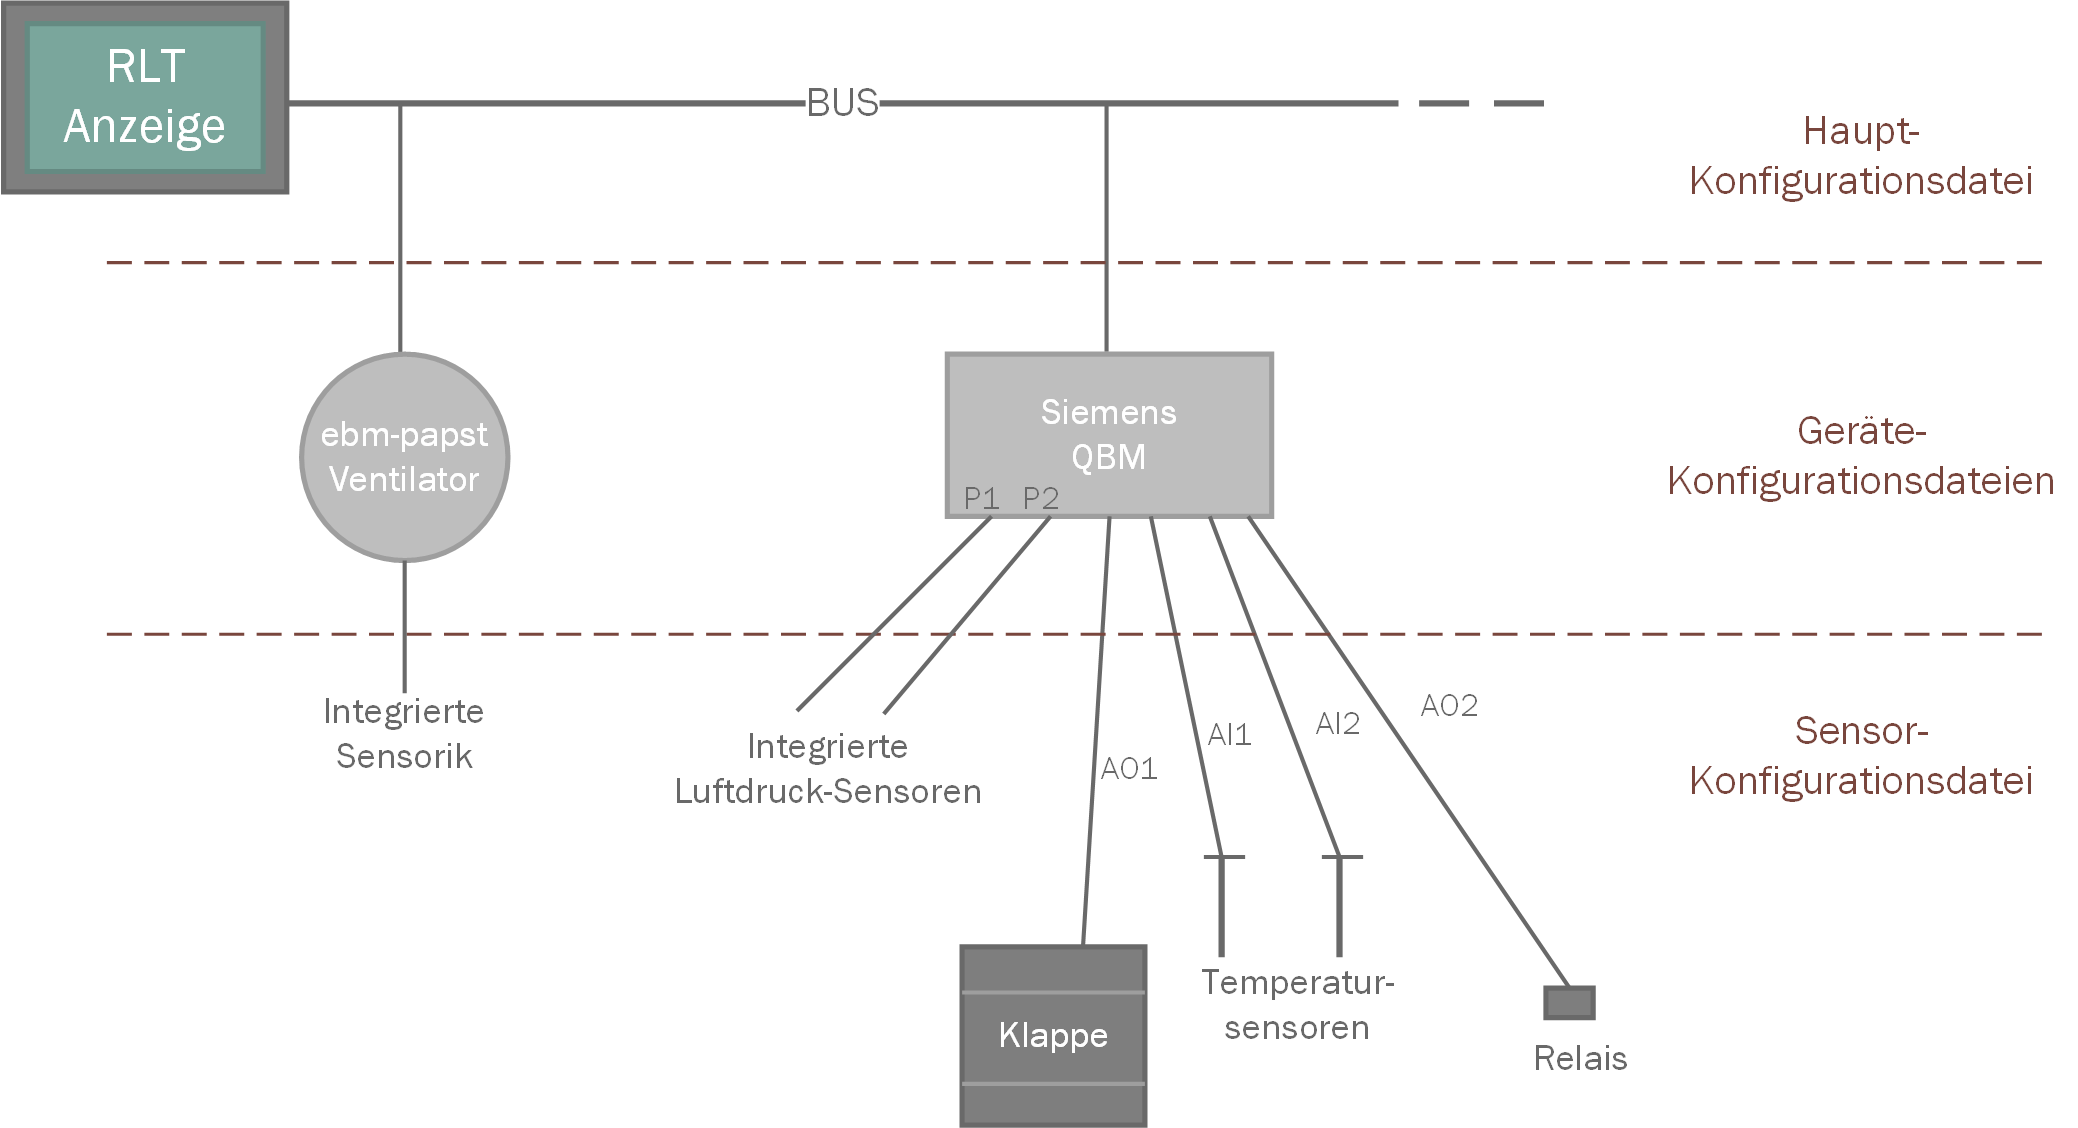
\includegraphics[width=\textwidth]{Komponenten_simpler_Aufbau_fuer_Dateikonzept}
	\caption{Vereinfachter Aufbau der Komponenten \label{fig:vereinfachter_aufbau_dateikonzept}}
\end{figure}

\newpage
Es folgt eine aufbauende Beschreibung und Erklärung der drei Dateitypen:
%Fenkart fragen, ob ich bei den Geräten auf seinen Teil verweisen kann
% Wer beschreibt baud_rate, register, adresse, function code \ref{modbus_funktionsweise}

\begin{enumerate}

	\item \textbf{Sensor-Konfigurationsdatei} (\enquote{sensors.json}): Es gibt kein explizites \gls{modbus} Register, um die Maßeinheit eines Messwerts zu übertragen. Deswegen muss die Maßeinheit der unterschiedlichen Sensorik aus Datenblättern entnommen und jeweils zugeordnet werden. Dazu dient die Sensor-Konfigurationsdatei, welche eine Liste aller Sensoren (\zB bestimmte Temperatursensoren) mit der jeweils dazugehörigen Maßeinheit beinhaltet. Komponenten wie Ventilatoren haben integrierte Sensoren. Auch in diesem Fall kann für die Maßeinheit ein Eintrag in die \enquote{sensors.json} Datei gemacht werden. 
	
	Die einfache Ergänzung neuer Sensoren ist der Zweck der Sensor-Konfigurationsdatei. Diese muss nur dann verändert werden, wenn ein neuer Sensortyp, der noch nicht in der Sensor-Konfigurationsdatei steht, ergänzt wird. 
	
	Jeder Eintrag der Sensor-Konfigurationsdatei hat zwei Parameter, welche in Tab. \ref{tab:sensors_json_parameter} zu sehen sind.
    
\begin{table}[h]
    \caption{Parameter der Sensor-Konfigurationsdatei (\enquote{sensors.json})}
    \label{tab:sensors_json_parameter}
    \begin{tabular}{p{\dimexpr 0.1\textwidth-2\tabcolsep} p{0.6\textwidth} | p{0.25\textwidth}}
        \toprule
        \textbf{Name} & \textbf{Beschreibung} & \textbf{Beispiel} \\
        \midrule
        type & Der Sensorname, auf den später in der Haupt-Konfigurationsdatei unter \enquote{type} referenziert wird. &  
        \begin{jsonTable}
"type": "NI1000"
        \end{jsonTable} 
        \\
        unit & Die Einheit des entsprechenden Sensors. (Diese muss auch in der Geräte-Konfigurationsdatei unter \enquote{units} vorhanden sein.) &  
        \begin{jsonTable}
"unit": "°C"
        \end{jsonTable} 
        \\
        \bottomrule
    \end{tabular}
\end{table}
	
		
	\item \textbf{Geräte-Konfigurationsdateien} (\zB \enquote{QBM97XX.json} oder \enquote{EBM.json}): Hier sind gerätespezifische Daten hinterlegt. Hauptsächlich welche Ausgabeports eine bestimmte Komponente (\zB ein Ventilator) besitzt, welche Einstellungen diese Ausgänge haben und \ggf welche Maßeinheiten die integrierten oder extern angeschlossenen Sensoren zurückgeben. 
	
	Weil in den \acsp{rltanlage} der Firma Bösch häufig die gleichen Komponenten verwendet werden, wurden spezielle Geräte-Konfigurationsdateien konzipiert. Diese Dateien können in der Haupt-Konfigurationsdatei beliebig oft referenziert werden, da sie einmalig für jedes Gerätemodell erstellt werden und nur selten Änderungen unterliegen. Das Hinzufügen einer neuen Geräte-Konfigurationsdatei ermöglicht zudem die einfache Integration einer neuen Komponente, beispielsweise eines Ventilators einer anderen Marke.
	
	Der Aufbau der Geräte-Konfigurationsdateien basiert auf einem \enquote{ports} Array. In dieses werden mithilfe der Parameter aus Tab. \ref{tab:ports_array_parameter} die erforderlichen Informationen eingetragen.
    
\begin{longtable}[h]{p{\dimexpr 0.18\textwidth-2\tabcolsep} p{0.50\textwidth} | p{0.27\textwidth}}
    \caption{Parameter des \enquote{ports} Array der Geräte-Konfigurationsdateien}
    \label{tab:ports_array_parameter}
    \\ \toprule
    \textbf{Name} & \textbf{Beschreibung} & \textbf{Beispiel}
    \\ \midrule
    \endfirsthead
    \caption{Parameter des \enquote{ports} Array der Geräte-Konfigurationsdatei (Fortsetzung)}
    %
    \\ \toprule
    \textbf{Name} & \textbf{Beschreibung} & \textbf{Beispiel}
    \\ \midrule
    \endhead
    %
    \midrule
    \multicolumn{3}{r}{{Fortsetzung auf der nächsten Seite}} 
    \\ \bottomrule
    \endfoot
    %
    \bottomrule
    \endlastfoot
    port      	& Bezeichnung des Ausgabeports. Wird im Falle eines Geräts mit externer Sensorik (\zB Siemens \gls{qbm}) in der Haupt-Konfigurationsdatei unter \enquote{port} referenziert. & 
    \begin{jsonTable}
"port": "AI1"
    \end{jsonTable} 
    \\
    register 	& \gls{modbus} Register (Erklärung in Kapitel \ref{modbus_funktionsweise}) in dem der jeweilige Messwert gespeichert ist \bzw welches ausgelesen werden soll. % Das Register muss dabei immer dezimal angegeben werden, da \gls{gls_minimalmodbus} die hexadezimale Eingabe nicht unterstützt. 
    & 
    \begin{jsonTable}
"register": 11
    \end{jsonTable} 
    \\
    function\_code 	& \gls{modbus} Function Code (Erklärung in Kapitel \ref{modbus_funktionsweise}), mit dem auf das vorher angegebene Register zugegriffen werden soll. %Die zwei meist verwendeten Function Codes sind \enquote{3} für Input Register und \enquote{4} für Holding Register. 
    & 
    \begin{jsonTable}
"function_code": 3
    \end{jsonTable} 
    \\
    units 	& Array in dem jeder möglichen Maßeinheit für den jeweiligen Ausgabeport eine Skalierung zugeordnet wird. Die Skalierung dient \zB dazu, dem Messwert die angemessene Anzahl von Dezimalstellen zuzuweisen, da diese über \gls{modbus} nicht übertragen werden (Funktionsweise in Kapitel \ref{auslesen_rlt_parameter} erklärt).
    
    Wird bei Ports weggelassen, deren Werte nur von Python Funktionen (Erklärung in Kapitel \ref{python_functions}) zur Weiterverarbeitung verwendet werden. 
    
    Die Parameter eines Objekts dieses Arrays sind in Tab. \ref{tab:units_array_parameter} zu sehen.  & 
    \begin{jsonTable}
"units": "[ ]"
    \end{jsonTable} 
    \\
\end{longtable}

	
\begin{table}[H]
    \caption{Parameter des Unterarray \enquote{units}}
    \label{tab:units_array_parameter}
    \begin{tabular}{p{\dimexpr 0.18\textwidth-2\tabcolsep} p{0.47\textwidth} | p{0.3\textwidth}}
        \toprule
        \textbf{Name} & \textbf{Beschreibung} & \textbf{Beispiel} \\
        \midrule
        unit      	& Die Maßeinheit, die aus der Sensor-Konfigurationsdatei referenziert wird. & 
        \begin{jsonTable}
"unit": "°C"
        \end{jsonTable} 
        \\
        scaling 	& Skalierung des Messwertes. Kann aus Datenblättern entnommen werden. & 
        \begin{jsonTable}
"scaling": 0.1
        \end{jsonTable} 
        \\
        \bottomrule
    \end{tabular}
\end{table}
		
	\item \textbf{Haupt-Konfigurationsdatei} (\enquote{main\_config\_file.json}):
	Wie in Kapitel \ref{gui_design} beschrieben, ist zur übersichtlichen Darstellung der Messwerte eine Aufteilung in mehrere Abschnitte bzw. Seiten erforderlich. Auf diesen Seiten werden jeweils sinngemäß Messwerte zusammengefasst. Die Konfiguration der Seiten erfolgt in der Haupt-Konfigurationsdatei mithilfe von zwei parallelen Arrays: dem \enquote{pages}-Array und dem \enquote{devices}-Array. 	
	
	Im \enquote{devices} Array werden alle Komponenten \bzw Quellen der \acs{rltanlage}, nämlich Ventilatoren und \gls{qbm}s (vgl. Abb. \ref{fig:vereinfachter_aufbau_dateikonzept}), aufgeführt, von denen Messwerte ausgelesen werden sollen. Die Parameter des \enquote{devices} Arrays sind in Tab. \ref{tab:devices_array_parameter} näher erläutert.

 \begin{longtable}{p{\dimexpr 0.15\textwidth-2\tabcolsep} p{0.52\textwidth} | p{0.28\textwidth}}
    \caption{Parameter des \enquote{devices} Array der Haupt-Konfigurationsdatei}
    \label{tab:devices_array_parameter}
    \\ \toprule
    \textbf{Name} & \textbf{Beschreibung} & \textbf{Beispiel}
    \\ \midrule
    \endfirsthead
    \caption{Parameter des \enquote{devices} Array der Haupt-Konfigurationsdatei (Fortsetzung)}
    %
    \\ \toprule
    \textbf{Name} & \textbf{Beschreibung} & \textbf{Beispiel}
    \\ \midrule
    \endhead
    %
    \midrule
    \multicolumn{3}{r}{{Fortsetzung auf der nächsten Seite}} 
    \\ \bottomrule
    \endfoot
    %
    \bottomrule
    \endlastfoot
    device     	& Angabe des Gerätetyps, indem auf den Namen der zugehörigen Geräte-Konfigurationsdatei referenziert wird. & 	
    \begin{jsonTable}
"device": "QBM97XX"
    \end{jsonTable}  
    \\
    id         	& Beliebig auswählbare, jedoch eindeutige Bezeichnung für das Gerät. Mit der \enquote{id} wird im \enquote{pages} Array auf das Gerät referenziert.  & 	
    \begin{jsonTable}
"id": "QBM1"
    \end{jsonTable}  
    \\
    baud\_rate	& Eingestellte Baudrate (vgl. Kapitel \ref{baud_rate}). Ist bei allen Komponenten einer \acs{rltanlage} gleich. & 	
    \begin{jsonTable}
"baud_rate": 19200
    \end{jsonTable}  
    \\
    mbaddress	& Die \gls{modbus} Adresse des Geräts. (vgl. Kapitel \ref{modbus_funktionsweise}) & 	
    \begin{jsonTable}
"mbaddress": 1
    \end{jsonTable}  
    \\
    parity	& Parität. Mögliche Werte: \enquote{even}, \enquote{odd} oder \enquote{none} (vgl. Kapitel \ref{modbus_uebertragungsarten}) & 	
    \begin{jsonTable}
"parity": "even"
    \end{jsonTable}  
    \\
    stop\_bits	& Anzahl der Stopbits einer Nachricht (vgl. Kapitel \ref{modbus_uebertragungsarten}) & 	
    \begin{jsonTable}
"stop_bits": 1
    \end{jsonTable}  
    \\
    zero\_based	& Gibt an, ob die \gls{modbus} Register von 0 oder 1 ausgehend gezählt werden. Mögliche Werte: \enquote{true} oder \enquote{false}.
    
    (Bemerkung: Bei Siemens \gls{qbm}s normalerweise \enquote{false}, bei ebm-papst Ventilatoren \enquote{true}) & 	
    \begin{jsonTable}
"zero_based": false
    \end{jsonTable}  
    \\
    sensors	& Array aller am Gerät angeschlossenen Sensoren. Bei Ventilatoren und Ausgabeports, deren Werte ausschließlich von Python Funktionen zur Weiterverarbeitung genutzt werden (Erklärung in Kapitel \ref{python_functions}), wird auf die Angabe verzichtet. 
    
    Die zwei Parameter, die für jedes Objekt dieses Arrays angegeben werden, sind in Tab. \ref{tab:sensors_array_parameter} zu finden. & 	
    \begin{jsonTable}
"sensors": [ ]
    \end{jsonTable}  
    \\
\end{longtable}
	
\begin{table}[H]
    \caption{Parameter des Unterarray \enquote{sensors}}
    \label{tab:sensors_array_parameter}
    \begin{tabular}{p{\dimexpr 0.12\textwidth-2\tabcolsep} p{0.53\textwidth} | p{0.3\textwidth}}
        \toprule
        \textbf{Name} & \textbf{Beschreibung} & \textbf{Beispiel} \\
        \midrule
        port   	& Verweist auf den Ausgabeport aus der Geräte-Konfigurationsdatei (siehe Tab. \ref{tab:ports_array_parameter}). Mögliche Werte können also \zB der Datei \enquote{QBM97XX.json} entnommen werden. & 	
        \begin{jsonTable}
"port": "AI1"
        \end{jsonTable}  
        \\
        type 	& Verweist auf einen Sensor aus der Sensor-Konfigurationsdatei. Mögliche Werte können also \zB der Datei \enquote{sensors.json} entnommen werden. & 	
        \begin{jsonTable}
"type": "LG-NI1000"
        \end{jsonTable}  
        \\
        \bottomrule
    \end{tabular}
\end{table}
	

	Im \enquote{pages} Array werden alle Seiten, die später auf der \acs{rltanzeige} veranschaulicht werden sollen, definiert. Dabei werden die in Tab. \ref{tab:devices_array_parameter} definierten Quellen den richtigen Seiten zugeordnet. Die Parameter des \enquote{pages} Array sind in Tab. \ref{tab:pages_array_parameter} notiert.
	
	% unterschiedliche anzahl der Komponenten

\begin{table}[H]
    \caption{Parameter des \enquote{pages} Array der Haupt-Konfigurationsdatei}
    \label{tab:pages_array_parameter}
        \begin{tabular}{p{\dimexpr 0.12\textwidth-2\tabcolsep} p{0.53\textwidth} | p{0.3\textwidth}}
        \toprule
        \textbf{Name} & \textbf{Beschreibung} & \textbf{Beispiel} \\
        \midrule
        title      	& Beliebig auswählbarer Titel der Seite. & 
        \begin{jsonTable}
"title": "Allgemein"
        \end{jsonTable} 
        \\
        sources 	& Array aller Messwerte, die auf einer Seite angezeigt werden sollen. Die Parameter, die in einem Objekt dieses Arrays benutzt werden, sind in Tab. \ref{tab:sources_array_parameter} zu sehen. & 
        \begin{jsonTable}
"sources": "[ ]"
        \end{jsonTable} 
        \\
        \bottomrule
    \end{tabular}
\end{table}

   
\begin{longtable}{p{\dimexpr 0.2\textwidth-2\tabcolsep} p{0.42\textwidth} | p{0.33\textwidth}}
    \caption{Parameter des Unterarray \enquote{sources}}
    \label{tab:sources_array_parameter}
    \\ \toprule
    \textbf{Name} & \textbf{Beschreibung} & \textbf{Beispiel}
    \\ \midrule
    \endfirsthead
    \caption{Parameter des Unterarray \enquote{sources} (Fortsetzung)}
    %
    \\ \toprule
    \textbf{Name} & \textbf{Beschreibung} & \textbf{Beispiel}
    \\ \midrule
    \endhead
    %
    \midrule
    \multicolumn{3}{r}{{Fortsetzung auf der nächsten Seite}} 
    \\ \bottomrule
    \endfoot
    %
    \bottomrule
    \endlastfoot
    port & Ein Array mit den Quellen, aus denen der Messwert ausgelesen wird. Dabei wird meistens nur ein Objekt mit \enquote{id} (siehe Tab. \ref{tab:devices_array_parameter}) des Geräts und \enquote{port} (siehe Tab. \ref{tab:ports_array_parameter}) angegeben. In einigen Szenarien ist es erforderlich, mehrere Quellen für abgeleitete Messwerte zu verwenden (siehe Kapitel \ref{python_functions}). In solchen Fällen werden dem Array zusätzliche Objekte hinzugefügt. &  
    \begin{jsonTable}
"port": [
    { "QBM1": "AI1" }
]
    \end{jsonTable} 
    \\
    description         & Beliebig auswählbare Bezeichnung für den Messwert. Der Messwert wird später auf der \acs{rltanzeige} so bezeichnet. & 
    \begin{jsonTable}
"description": "Temperatur Zuluft"
    \end{jsonTable}  
    \\
    python\_function    & (Optionaler) Parameter, der nur angegeben wird, wenn der jeweilige Messwert abgeleitet berechnet werden muss. (Erklärung in Kapitel \ref{python_functions}). & 
    \begin{jsonTable}
"python_function": "relay_position"
    \end{jsonTable} 
    \\
    additional\_info    & (Optionaler) Parameter, der nur angegeben wird, falls die jeweilige Python Funktion zusätzliche Informationen benötigt. (Erklärung in Kapitel \ref{python_functions}). & 
    \begin{jsonTable}
"additional_info": { "switching_voltage": 5 }
    \end{jsonTable} 
    \\
\end{longtable}
					
\end{enumerate}

%Bedienungsanleitung für Servicetechniker erwähnen
Zuletzt ist zu erwähnen, dass Servicetechnikerinnen und Servicetechniker zur Installation einen Ordner bekommen. Darin befindet sich eine Vorlage für die \enquote{main\_config\_file.json} Datei, welche im Normalfall die einzige Datei sein sollte, die bearbeitet bzw. verändert wird.
In einem Unterordner (\enquote{devices}) sind Geräte-Konfigurationsdateien und die Sensor-Konfigurationsdatei zu finden. Diese Dateien müssen, wie gerade erwähnt, nur verändert werden, wenn noch nie verwendete Komponenten, wie z.B. eine neue Art von Ventilator oder Sensor, in der \acs{rltanlage} verbaut werden.

Ein Beispiel zu allen Dateitypen ist im Anhang zu finden.




